\chapter{АЛГОРИТМ МОДУЛЯ СКАНИРОВАНИЯ}\label{chap:algorithms}
    \section{Этапы работы алгоритма}
        Задача алгоритма заключается в преобразовании входных данных -- видео процесса сканирования и dxf файла с заданным контуром -- в gcode файл. Gcode файл это последовательность инструкций для принтера написанных особым образом. Файл формата dxf это векторное изображение некоторого произвольного рисунка, которое необходимо нанести на изделия в сцене.
        В целом алгоритм модуля состоит из следующих операций:
        \begin{enumerate}
            \item Обработка видео/Получение облака точек
            \item Поиск объектов в облаке
            \item Генерация gcode файла
        \end{enumerate}
        
        Последовательность операций отражена в блок-схеме на рисунке \ref{pic:general_scheme}.
        \begin{figure}[!ht]
            \centering
            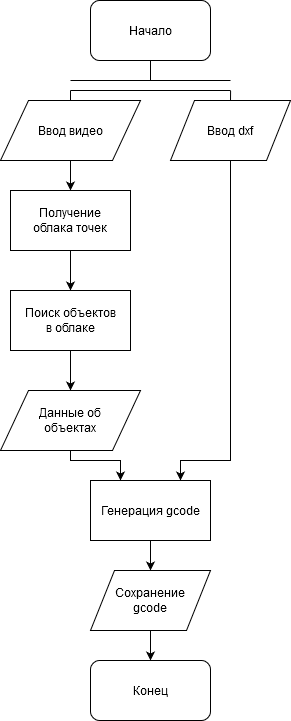
\includegraphics[width=0.4\linewidth]{general scheme}
            \caption{Обобщённая блок схема алгоритма модуля}
            \label{pic:general_scheme}
        \end{figure}
         При запуске алгоритма на вход передаются видео со сканера и dxf файл. После этого запускаются этапы обработки видео и dxf файла. Эти этапы независимы друг от друга и могут выполняться параллельно. Этап обработки видео включает в себя предобработку каждого кадра, затем выделение лазера в кадре, расчёт координат по формулам из главы \ref{chap:math}. Результатом этого этапа является облако точек сцены. Оно передаётся в следующий блок для поиска объектов. Цель этого этапа в получении положений и ориентаций объектов в сцене. Затем данные об объектах и подготовленный рисунок передаются в последний блок алгоритма, где из них генерируется файл инструкций для принтера которые задают последовательность печати рисунка из dxf файла на каждый найденный объект в сцене.
    \section{Блок обработки видео}
        Как уже было сказано, блок обработки видео включает в себя следующие шаги, которые выполняются для каждого кадра видео:
        \begin{enumerate}
            \item Предобработка кадра
            \item Выделение лазера
            \item Расчёт координат
        \end{enumerate}
        
        \begin{wrapfigure}{r}{0.5\linewidth}
            \centering
            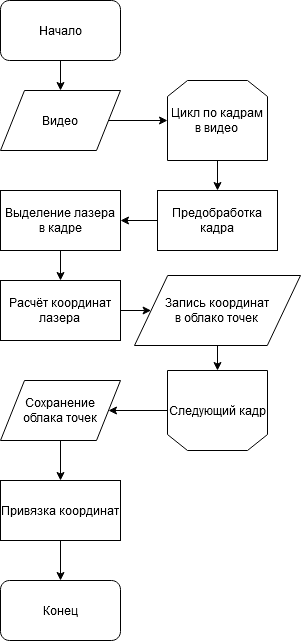
\includegraphics[height=0.45\textheight, keepaspectratio]{video_processing}
            \caption{Обобщённая блок схема обработки видео}
            \label{pic:video_processing}
        \end{wrapfigure}
        После этого облако точек сохраняется в памяти и производится привязка координат к системе принтера. Этот этап необходим, потому что в виду аппаратных ограничений сканирование в общем случае начинается в произвольном месте до рабочей поверхности и получить точную координату не представляется возможным.
        \sloppy Результатом работы алгоритма становится облако точек, представляющее из себя матрицу размерностью $ (\mbox{\textit{количество кадров}}\times\mbox{\textit{ширина кадра}}) $ где в каждой ячейке записана координата соответствующая этой точке. Таким образом облако точек одновременно является картой глубины сцены.
        
        \subsection{Предобработка}
            \begin{wrapfigure}{l}{0.42\linewidth}
                \centering
                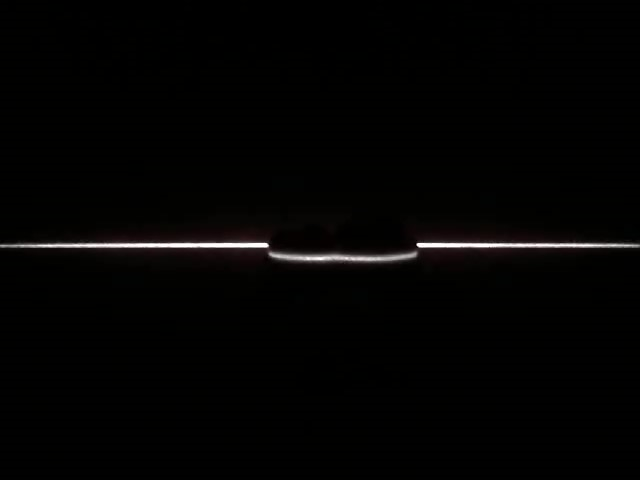
\includegraphics[width=0.4\textwidth]{frame_sample}
                \caption{Пример кадра из видео}
                \label{pic:frame_sample}
            \end{wrapfigure} 
            Перед тем как выделить на изображении лазер, необходимо провести предобработку, которая сгладит шумы в кадре и уберёт большинство лишней информации. Первым шагом необходимо обрезать видео по заранее установленной области интереса. Вне этой области заранее гарантировано отсутствие полезной информации, т.е. вне этой области нет рабочей зоны. 
            
            Затем к изображению применяется фильтр гаусса. Он представляет собой операцию свёртки гауссовой функцией на изображении. Применение фильтра гаусса позволяет снизить влияние шумов на изображении, что поможет на следующем шаге. Побочным эффектом фильтра является размытие изображения\cite{Corke2017}.
            
            После этого с полученного изображения снимается <<маска>> -- то есть изображение бинаризируется. В таком изображении единицами обозначена область, которую необходимо оставить, а нулями -- отбросить. Для получения маски предусмотрено два подхода на выбор -- бинаризация по заданному пороговому значению и бинаризация с порогом по Оцу. Последняя хороша тем, что позволяет избежать необходимость ручного подбора порогового значения. 
            
            Метод Оцу применим к изображениям на гистограмме которых есть только два пика. Хорошее пороговое значение для таких изображений находится между этими двумя пиками\cite{opencvTHRESH}.
            
            Это идеально подходит для нашего случая. Такая маска единицами пометит области на изображении, в которых с наибольшей вероятностью находится лазер, а нулями области, где лазера почти наверняка нет.
            
            Последним шагом является применение маски к обрезанному изображению, что представляет собой простое поэлементное умножение. Таким образом получается изображение, в котором область, где почти наверняка лазера нет, состоит из пикселей значение которых равно нулю, остальная же часть остаётся нетронутой.

            Это изображение затем передаётся в следующий блок алгоритма для выделения лазера.

        \subsection{Выделение лазера}
            Для постановки задачи выделения лазера в первую очередь необходимо определить, что из себя представляет линия лазера на изображении. В нашем случае линия лазера в кадре располагается параллельно оси $ X $ изображения. Интенсивность в профиле лазера, т.е. сечении в перпендикулярном линии направлении, соответствует Гауссовому распределению\cite{Qi2013, Molder2014} с некоторым шумом. Пик интенсивности, без учета шума, соответствует центру полосы лазера.
            \begin{wrapfigure}{l}{0.4\linewidth}
                \centering
                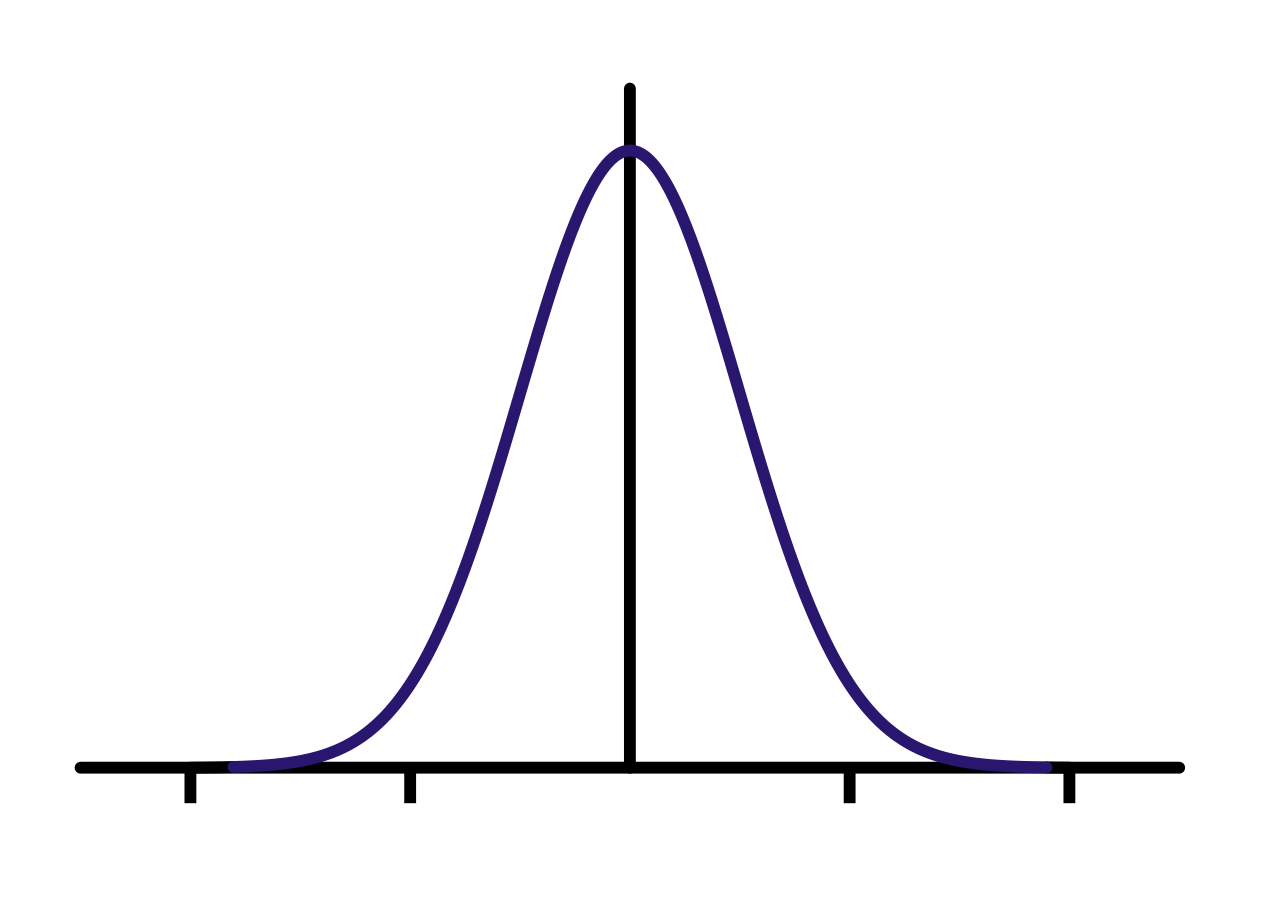
\includegraphics[width=0.38\textwidth]{gauss_profile}
                \caption{Распределение Гаусса}
                \label{pic:gauss_profile}
            \end{wrapfigure}
            Таким образом задача выделения лазера на изображении в первом приближении сводится к определению пика интенсивности для каждого профиля лазера, то есть в нашем случае для каждой колонки пикселей изображения.
            
            Однако задача усложняется наличием шумов на изображении, которые постоянно искажают профиль интенсивности лазера. Причинами шумов могут являться светочувствительный сенсор в камере, нежелательные отражения света лазера от поверхности, неподходящие условия окружения, программная обработка изображения на этапе кодирования-декодирования и так далее.
            
            Помимо этого в общем случае линия лазера на изображении не является непрерывной. Разрывы могут возникать в следствии недостаточной контрастности лазера или попадания линии лазера в слепую зону. Некоторые методы достраивают недостающие участки лазера с помощью аппроксимации, другие не обрабатывают эти области.
            
            Рассмотрим некоторые из существующих алгоритмов для выделения лазера и следующие их характеристики.
            
            \noindent{%
            \textit{\underline{Точность}} -- с какой точностью определяется положение лазера. Может быть \textbf{\textit{пиксельная}} -- положение определяется с точностью до одного пикселя -- и \textbf{\textit{субпиксельная}} -- положение определяется с точностью в доли пикселя\\
            \textit{\underline{Восприимчивость к шуму}} -- критично ли наличие шумов на изображении для работы алгоритма\\
            \textit{\underline{Требования к вычислительным мощностям}} -- зависит от сложности операций и их количества.}
            
            \paragraph{Метод максимумов}
                Данный метод находит максимум интенсивности в каждой колонке изображения и считает его центром лазера. Этот метод обладает пиксельной точностью. На работу данного метода влияют значительные шумы, как правило, связанные с окружением и поверхностью сканирования. Не требует серьёзных вычислительных мощностей, поскольку операция поиска максимума в колонке одна из простейших.
            
            \paragraph{Laplacian of Gaussian}
                На реальных изображениях пик профиля лазера как правило срезан, поэтому метод максимумов в данном случае не даёт максимальной точности\cite{Molder2014}. 
                
                Чтобы это преодолеть, к изображению можно использовать LoG преобразование, то есть применить свёртку гауссовой функцией на изображение, после чего вычислить вторую производную по изображению. Полученный результат инвертировать. На полученном новом изображении пики соответствуют центру лазера. 
                
                \begin{wrapfigure}{r}{0.4\linewidth}
                    \centering
                    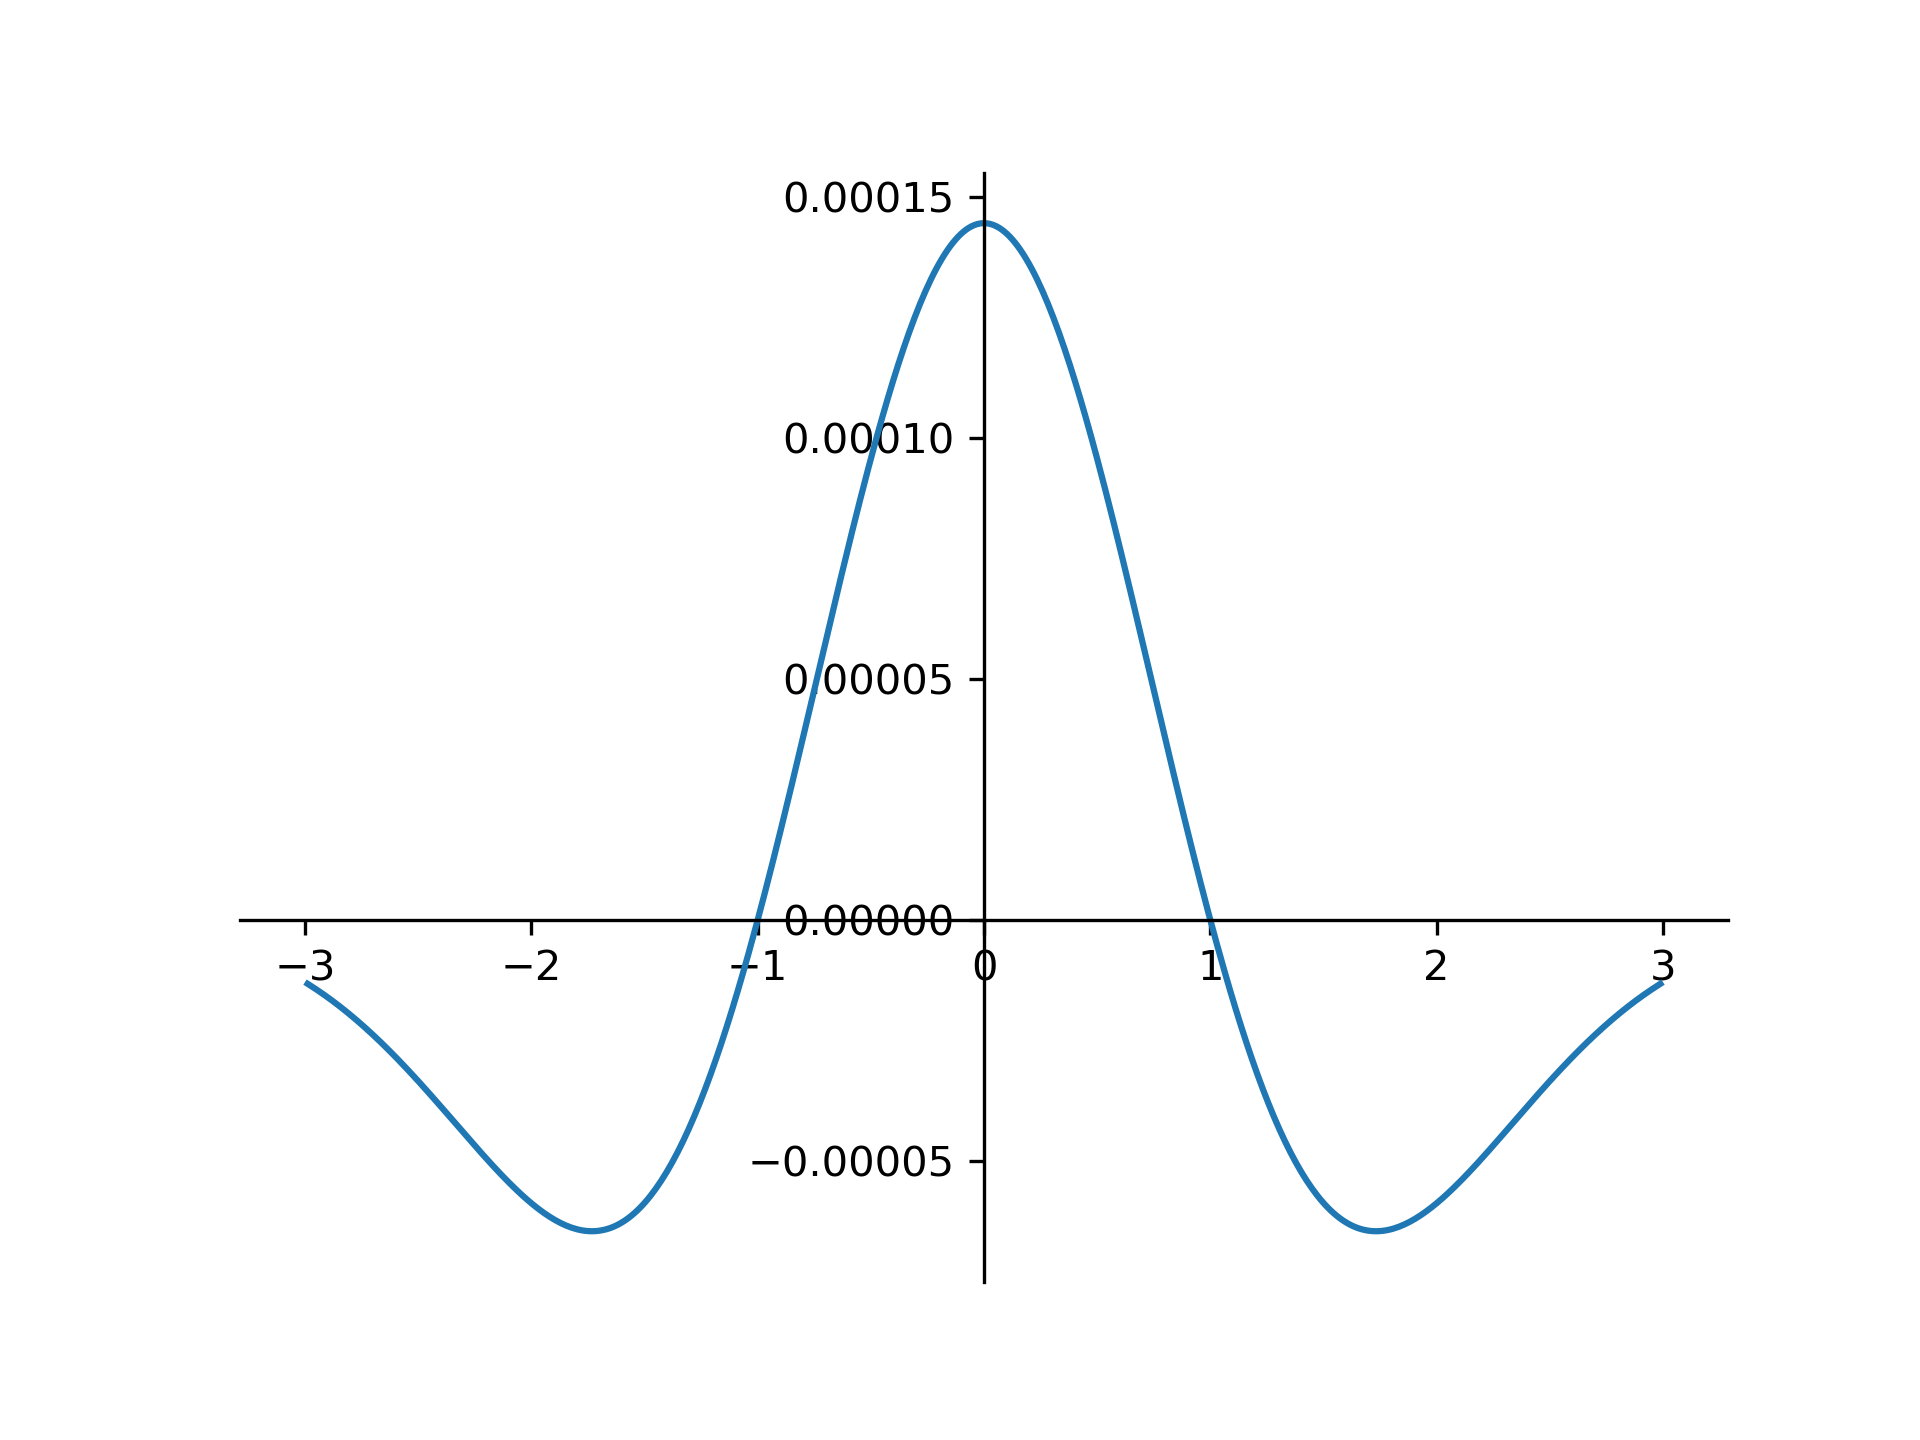
\includegraphics[width=0.38\textwidth]{gauss_second_order}
                    \caption{Профиль интенсивности лазера после LoG преобразования}
                \end{wrapfigure}
                Данный метод в общем случае используется для выделения краёв и линий на изображении\cite{Steger2000}. Для использования этого метода необходимо выбрать дисперсию $ \sigma $ гауссового распределения и окно свёртки. При малых $ \sigma $ таким образом возможной найти линии малой толщины, при б\'{о}льших $ \sigma $ наоборот, но одновременно за одно преобразование найти линии сильно отличающейся толщины невозможно. Параметр $ \sigma $ можно найти эмпирически, но можно воспользоваться оценкой $ \sigma > \dfrac{w}{\sqrt{3}} $ из работы \cite{Steger2000}, где $ w $ -- ширина линии лазера в пикселях.
                
                Данный метод также обладает пиксельной точностью. Более устойчив к шумам на изображении из-за использования гауссового размытия, что, однако, ухудшает выделение лазера на краях объектов. Из-за LoG преобразования данный метод требует больших вычислительных ресурсов, чем метод максимумов и, соответственно, выполняется медленнее.
            
            \paragraph{Квадратичная аппроксимация}
                Предыдущие два метода возможно улучшить и привести точность к субпиксельной\cite{Molder2014}. Если рассмотреть профиль интенсивности лазера по пикселям, то в общем случае действительный максимум приходится на значение между пикселей. Также можно заметить что в окрестности максимума профиль представляет собой некоторую параболу $ y = ax^2 + bx + c $. Взяв три точки -- точку перед максимумом, точку максимума, точку после максимума -- легко найти коэффициенты этой параболы и, соответственно, вершину, которая будет являться действительным максимумом.
                
                Данный метод лучше применим к LoG трансформации, т.к. уже было сказано, что изначальный профиль лазера как правило обрезан при вершине. Однако в определённых условиях можно применять данный подход и для метода максимумов.
                
                Применение этого метода увеличивает требование к вычислительным мощностям, однако незначительно, так как вычисления относительно просты и легко оптимизируемы.
            
            \paragraph{Метод центра масс (Gray-Gravity Method)}
                По данному методу центр лазера $ (i_c, j_c) $ рассчитывается как <<центр масс>> интенсивностей в колонке $ j_c $ изображения по формуле
                \begin{equation}
                    i_c = \left(\sum\limits_{i=1}^{H}I(i, j_c)\cdot i\right)\cdot\left(\sum\limits_{i=1}^{H}I(i, j_c)\right)^{-1}
                \end{equation}
                где $ H $ -- высота кадра в пикселях, $ I(i, j_c) $ интенсивность $ i-\textit{го} $ пикселя в колонке.
                
                
                Данный метод обладает субпиксельной точностью\cite{Li2017}. Однако, он крайне чувствителен к шумам, поэтому несмотря на субпиксельную точность его применение в задачах требующих высокой точности нежелательно. При этом данный метод один из самых быстрых и нетребовательных к вычислительным мощностям в виду тривиальности вычислений.
                
            \paragraph{Улучшенный метод центра масс (Improved Gray-Gravity Method)}
                Улучшенный вариант предыдущего метода\cite{Li2017}. Предполагает два основных шага -- предварительное определение центра лазера методом центра масс, затем уточнение координаты.
                
                Уточнение координаты происходит следующим образом:
                С помощью методом скользящих наименьших квадратов находится касательная, нормаль и кривизна линии в точке предварительного центра. На основе этих значений подбирается прямоугольная область ограничивающая множество точек для расчётов. Затем рассчитывается отклонение действительного центра лазера от предварительного на основе интенсивности точек в регионе и их расстояния до линии пересекающей предварительный центр по направлению касательной в этой точке.
                
                Достоинством этого метода является то, что он учитывает направление линии лазера в кадре и кривизну линии. Предыдущие методы предполагают что лазер параллелен оси $ x $ изображения, из-за чего теряют в точности в виду искажения распределения интенсивности.
                
                Данный метод обладает субпиксельной точностью и не настолько чувствителен к шумам как обычный метод центра масс. Также предварительным шагом можно применять любой другой метод. Однако данный метод сложнее реализовать и он более требователен к вычислительным мощностям, чем предыдущие методы.
                
            \paragraph{Другие методы}
                Кроме упомянутых методов существуют множество других. В частности \textit{Gaussian Fitting}\cite{Qi2013} и \textit{Usamentiaga Method}\cite{Usamentiaga2012}.
                
                Gaussian Fitting основан на методе Штегера, описанном в работе \cite{Steger2000}. В работе \cite{Qi2013} выдвигается математический аппарат для определения параметров распределения лазера на основе данных с изображения, в частности соотношения сигнал/шум.
                
                Суть данного метода заключается в том, чтобы отыскать реальное распределение интенсивности лазера на изображении без влияния шума и таким образом найти реальный центр лазера.
                
                Достоинствами этого метода являются высокая устойчивость к шумам и высокая точность определения центра лазера.
                
                Недостатком является большое время выполнения даже для одного изображения, что не позволяет использовать этот метод в задачах требующих быстрого выполнения, а также значительная сложность реализации алгоритма.
                
                Usamentiaga method решает задачу выделения лазера в сложных индустриальных условиях и представляет алгоритмы устойчивые к шумам и нежелательным отражениям лазера. Также метод интересен тем, что предлагает алгоритм заполнения зон, где выделение лазера не удалось. В своей основе данный метод представляет комбинацию метода максимумов и метод центра масс, применённый в окрестности максимума.
                
                Данный метод относится к субпиксельным и очень устойчив к шумам различного характера. При этом точность определения лазера не уступает gaussian fitting при значительно меньшем требовании к вычислительным мощностям. По данным работы \cite{Li2017} данный метод в 90 раз быстрее gaussian fitting, но в 3 раза медленнее метода центра масс. Это позволяет использовать его в задачах требующих малого времени выполнения. Однако он также как и gaussian fitting сложен в реализации.
            
            \paragraph{Выбранный метод}
                В конечном итоге основным был выбран метод Laplacian of Gaussian в комбинации с квадратичной аппроксимации описанный в статье \cite{Molder2014}, поскольку он обладает наиболее оптимальными характеристиками работы и время выполнения сканирования для видео из 1240 кадров (длительность 40 секунд с частотой 30 кадров в секунду) составляет около 10 секунд, что удовлетворяет техническому заданию.
            
        \subsection{Привязка координат}
            Ранее было сказано, что в виду аппаратных ограничений видео сканирования в общем случае начинается в неопределённый момент перед рабочей зоной. При этом нет возможности узнать координату сканера в момент начала записи видео. Это порождает проблему несоответствия рассчитанных в процессе обработки координат и реальных. Таким образом необходимо разработать алгоритм, который позволял бы по данным с видео определить необходимое смещение координат.
            
            Основная идея такого алгоритма состоит в том, что необходима уникальная метка-идентификатор, имеющая заранее известную координату. Такая метка и алгоритм должны удовлетворять следующим требованиям:
            \begin{itemize}
                \item Лёгкое определение по входному видео
                \item Устойчивость к ложноположительным срабатываниям
                \item Лёгкое внедрение в конструкцию
                \item Минимальное влияние на общее время работы алгоритма
            \end{itemize}

            Предлагается использовать рельефные идентификаторы на столе, которые будут образовывать некоторый паттерн схожий с идеей штрихкода. Таким образом после сканирования в облаке точек сцены будет видна данная метка, которую возможно распознать программными методами и рассчитать необходимое смещение.
            
            В конечном итоге идентификатор представляет собой ряд меток (рисунок \ref{pic:mark}) расположенных на некотором заданном расстоянии друг от друга. Метки же в свою очередь представляют некоторую прямоугольную поверхность заданной ширины на определённой высоте от стола. Высота от стола для всех меток одинаковы, остальные параметры произвольны.
            
            \begin{figure}[H]
                \centering
                \includegraphics[width=0.5\linewidth]{mark}
                \caption{Рельефная метка}
                \label{pic:mark}
            \end{figure}
            
            Алгоритм перебирает профили сцены в облаке точек и сравнивает их на соответствие заданному идентификатору. Как только алгоритм находит подходящий профиль рассчитывается необходимое смещение, которое применяется ко всем координатам в облаке.
            
    \section{Блок поиска объектов}
        Задача поиска объектов в произвольном облаке точек одна из сложнейших. Такие задачи в настоящее время пытаются решить с использованием нейронных сетей и <<искусственного интеллекта>>. На данный момент нет стандартных подходов к решению этой задачи.
        
        Однако в нашем случае задача значительно упрощается по следующим причинам:
        \begin{itemize}
            \item имеется карта глубины с прямым соответствием пикселей и реальных координат
            \item объекты относительно простые
            \item необходимо распознать только верхнюю часть объектов
        \end{itemize}
        Поэтому возможно перевести задачу из распознавания объектов в пространстве в распознавание замкнутых контуров на изображении.
        
        На вход алгоритму подаётся карта глубины сцены, на которой видны изделия. Применив к изображению алгоритм watershed найдём контур для каждого объекта, даже в случае их прямого соприкосновения. 
        
        Данный алгоритм рассматривает изображение как топографическую карту, в которой высокая интенсивность обозначает пики, а низкая долины. Данный рельеф заполняется водой разных цветов (маркеры), начиная с изолированных долин. В местах смешивания выстраиваются барьеры. Этот процесс происходит до тех пор, пока все пики не окажутся под водой. Полученные таким образом водоёмы разных цветов обозначают различные контуры изображения\cite{opencvWATERSHED}.
        
        Поскольку карта глубины даёт прямое соответствие между пикселями и координатами, то наш контур задаётся некоторым пространственным многоугольником. Отбросив $ z $ координату, получим проекцию контура на плоскость. Затем можно рассчитать моменты этого контура и получить его центроиду. Так же через моменты можно найти ориентацию контура в пространстве (поворот вокруг центра), это эквивалентно вписыванию эллипса в контур и нахождения угла наклона главной диагонали.
        
        Момент $ m_{pq} $ контура можно посчитать по следующей формуле
        \begin{equation}
            m_{pq} = \sum\limits_{k}^{n}i_k^p j_k^q,
        \end{equation}
        где $ p $ и $ q $ -- порядки момента;\\
        $ \left(i_k, j_k\right) $ -- координаты вершины контура, пиксели или миллиметры;\\
        $ n $ -- количество вершин контура;\\
        Центр контура рассчитывается по формуле
        \begin{equation}
            (i_c,j_c) = \left(\dfrac{m_{10}}{m_{00}}, \dfrac{m_{01}}{m_{00}}\right)
        \end{equation}
        Угол ориентации в пространстве рассчитывается по формуле
        \begin{equation}
            \theta = \dfrac{1}{2}\arctan\left(\dfrac{b}{a-c}\right) + \left(a\le c\right)\dfrac{\pi}{2},
        \end{equation}
        где $ a = \dfrac{m_{20}}{m_{00}} - i_c^2 $; 
        $ b = 2\dfrac{m_{11}}{m_{00}} - i_cj_c $; 
        $ c = \dfrac{m_{02}}{m_{00}} - j_c^2 $
        
        Таким образом для каждого найденного контура программой формируется объект содержащий следующие данные:
        \begin{itemize}
            \item область в облаке точек, содержащую только этот контур
            \item координату центра объекта в плоскости
            \item ориентацию объекта в плоскости
        \end{itemize}
        Область в облаке сохраняется с целью оптимизации по времени алгоритма проекции рисунка на рельеф.
        
        На рисунке \ref{pic:contour_detection} изображён пример работы алгоритма для случая одного объекта. Видно, что некоторые детали на краях изделия пропадают. Это происходит из-за использования морфологических операций при предобработке до применения алгоритма watershed. Однако, это не мешает определить необходимые параметры объекта, т.к это происходит равномерно и симметрично по периметру объекта.
        
        \begin{figure}[H]
            \begin{subfigure}{0.5\linewidth}
                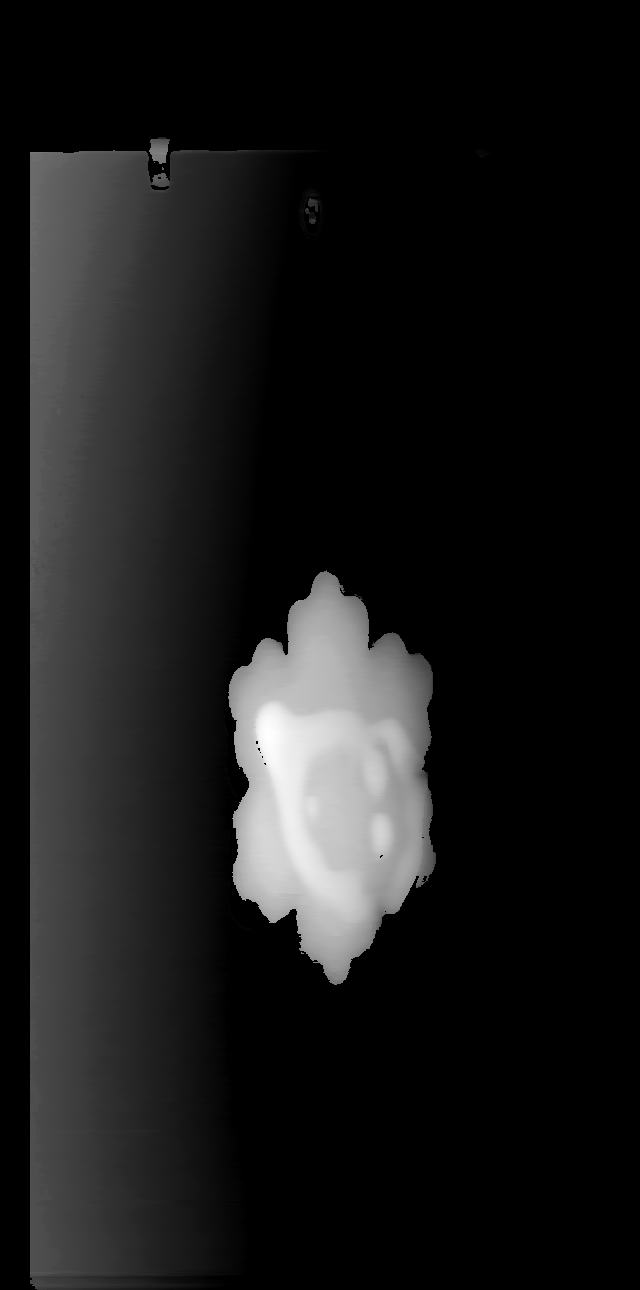
\includegraphics[width=\linewidth, trim={0, 7cm, 0, 12cm}, clip]{depthmap}
                \caption{Карта глубины поданная на вход}
            \end{subfigure}
            \begin{subfigure}{0.5\linewidth}
                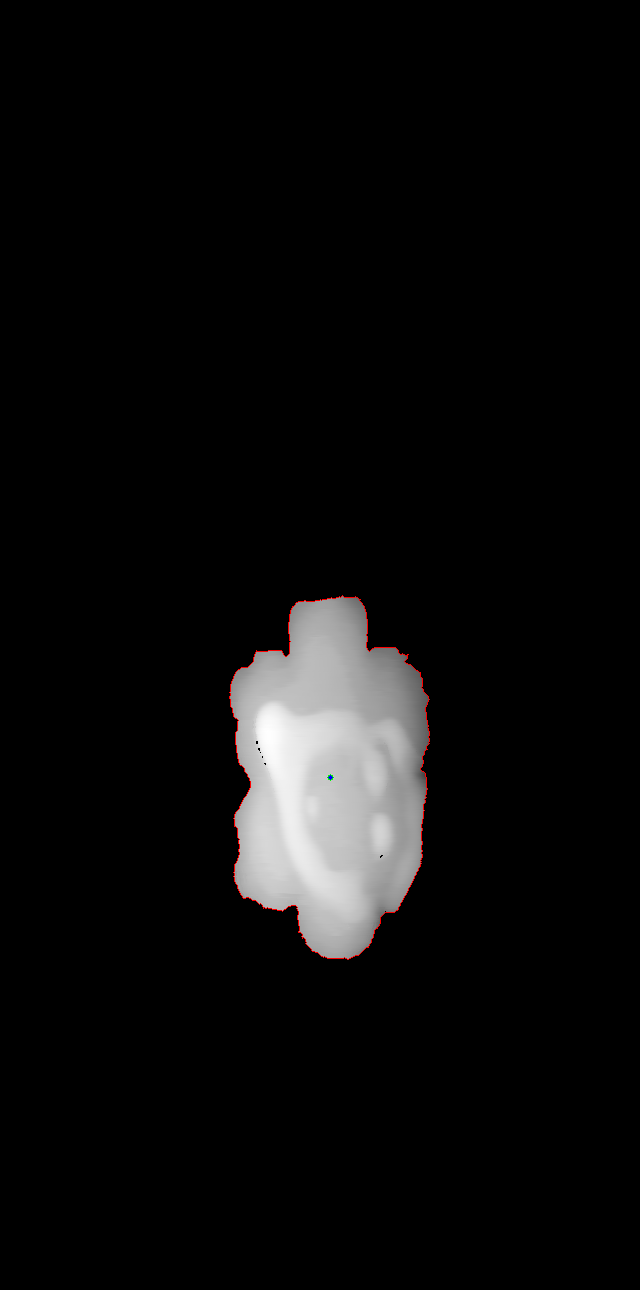
\includegraphics[width=\linewidth, trim={0, 7cm, 0, 12cm}, clip]{found_objects}
                \caption{Обнаруженные объекты}
            \end{subfigure}
            \caption{Пример работы алгоритма}
            \label{pic:contour_detection}
        \end{figure}
        
    \section{Блок генерации gcode}
        3D-принтеры, и прототип в частности, не способны описывать сложные кривые в пространстве. Возможно описывание окружностей и, в некоторых случаях, простейших сплайнов только в горизонтальной плоскости. Это существенное препятствие в нашем проекте, так как сопло печатающего элемента должно огибать сложную поверхность. Также dxf рисунок может задавать контуры сложной формы даже в плоскости. Для преодоления данных ограничений было решено реализовать слайсер-алгоритм решающий эту задачу.
        
        \begin{figure}[H]
            \centering
            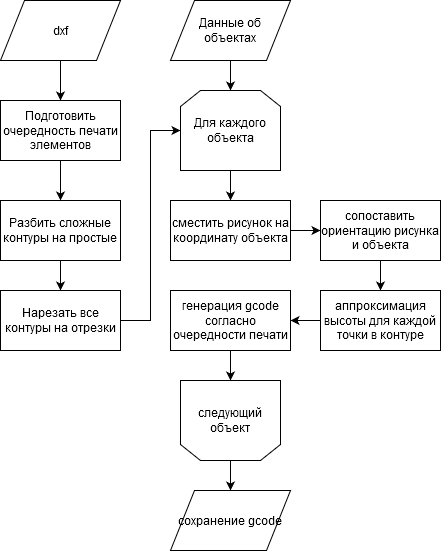
\includegraphics[width=0.5\linewidth]{gcoder}
            \caption{Блок-схема генератора gcode}
            \label{pic:gcoder}
        \end{figure}
        
         На вход алгоритма поступают данные об объектах и рисунок. В первую очередь происходит обработка dxf файла -- формируется очерёдность нанесения элементов рисунка в зависимости от их примыкания и расположения в структуре файла; сложные элементы (например, сплайны) разбиваются на более простые; все элементы <<нарезаются>> на отрезки определённой длины, заданной пользователем.
         
         Затем обработанный файл комбинируется с данными о каждом объекте. Для каждой точки в контуре аппроксимируется соответствующая высота на основе данных облака. В процессе разработки были опробованы три варианта аппроксимации -- выбор ближайшей точки, среднее \textit{k}-ближайших соседей и метод скользящих средних квадратов. Проиллюстрируем работу алгоритмов на примере dxf-файла изображённом на рисунке \ref{pic:dxf}.
                         
         \begin{figure}[!ht]
             \centering
             \includegraphics[width=0.4\linewidth]{dxf}
             \caption{Пример рисунка для нанесения}
             \label{pic:dxf}
         \end{figure}
         
         \paragraph{Ближайшая точка}
         По данному методу для заданной $ (x_p,y_p) $ координаты в облаке ищется аппроксимирующая точка $ (x_a, y_a, z_a) $ для которой $ (x_a-x_p)^2 + (y_a-y_p)^2 $ есть минимум среди всех точек в облаке.
         
         \begin{figure}[H]
             \centering
             \includegraphics[width=0.5\linewidth]{slicing_fine_nearest}
             \caption{Метод ближайшей точки}
             \label{pic:slicing_nearest}
         \end{figure}
         
         \paragraph{\textit{k}-ближайших соседей}
         По данному методу выбирается \textit{k} точек, расстояние до проекции которых от необходимой точки минимально. Затем вычисляется среднее координаты $ z $ этих точек. Полученное значение является аппроксимированной высотой искомой точки.
         
         \begin{figure}[H]
             \centering
             \includegraphics[width=0.5\linewidth]{slicing_fine_knn}
             \caption{Метод $ k $-соседей; $ k=30 $}
             \label{pic:slicing_knn}
         \end{figure}
         
         \paragraph{Скользящие наименьшие квадраты}
         Это метод поиска некоторой полиномиальной функции, которая аппроксимирует данные с наименьшей квадратичной ошибкой в окрестности заданной точки \cite{Veerabhadra2017}. То есть имея множество $ n $ точек $ \{M_i(x_i, y_i, z_i)\}_{i=1}^{n} $ и опорную точку $ M_p(x_p, y_p) $ необходимо найти коэффициенты $ c_{kl} $ следующей функции
         \begin{equation}
             f(x,y)=\sum\limits_{k=0}^{p}\sum\limits_{l=0}^{q}c_{kl}x^ky^l,
         \end{equation}
         где $ p $, $ q $ -- максимальная степень $ x $ и $ y $ переменных соответственно.
         Для нахождения коэффициентов необходимо решить задачу минимизации следующей функции
         \begin{equation}
             E = \sum\limits_{i}^{n}w_i(r_i)\left(\sum\limits_{k=0}^{p}\sum\limits_{l=0}^{q}c_{kl}x_i^k y_i^l - z_i\right),
         \end{equation}
         где $ w_i $ -- весовой коэффициент задающийся следующим образом
         \begin{equation}
            w_i(r_i) = 
                     \begin{cases}
                         1-6r_i^2+8r_i^3-3r_i^4, &r_i \le 1\\
                         0, &r_i > 1
                     \end{cases}
         \end{equation}
         где $ r_i $ -- нормализованное расстояние между опорной точкой $ M_p $ и точками $ M_i $ из множества, рассчитываемое по формуле
         \begin{equation}
             r_i = \sqrt{(x_i-x_p)^2 + (y_i-y_p)^2}\cdot R^{-1},
         \end{equation}
         где $ R $ -- радиус влияния, точки не входящие в этот радиус не имеют эффекта на аппроксимацию.
         Уравнения весовых коэффициентов выведены в работе \cite{LI2008}
         Минимизируя $ E $ и переписывая в матричном виде получаем следующее уравнение для коэффициентов функции $ f(x,y) $
         \begin{equation}
             c = \left[B^T W(M_p) B\right]^{-1} B^T W(M_p) z,
         \end{equation}
         где $ z = [z_1 ... z_n]^T$ -- вектор значений координат точек множества, $ B $ -- обобщённая матрица Вандермонда данных из $ (x,y) $ координат точек множества, в данном случае
         \begin{equation}
             B = 
             \begin{bmatrix}
                 1 & y_1 & x_1 & \cdots & x_1^p y_1^q\\
                 1 & y_2 & x_2 & \cdots & x_2^p y_2^q\\
                 \vdots & \vdots & \vdots & \ddots & \vdots\\
                 1 & y_n & x_n & \cdots & x_n^p y_n^q
             \end{bmatrix}
         \end{equation}
         
         \begin{figure}[H]
             \centering
             \includegraphics[width=0.5\linewidth]{slicing_fine_mls}
             \caption{Метод скользящих наименьших квадратов}
             \label{pic:slicing_mls}
         \end{figure}
         
         Найдя таким образом аппроксимацию поверхности легко вычислить координату $ z $ искомой точки.
        
        \paragraph{Выбранный метод}
            Из трёх методов предпочтительным является метод скользящих наименьших квадратов. Данный метод, как правило, применяется для восстановления сложных поверхностей по облаку точек. Он является более плавным и точным, чем остальные методы, что легко видно по рисункам \ref{pic:slicing_nearest}-\ref{pic:slicing_mls}. Однако данный метод значительно требовательнее к вычислительным мощностям, поэтому его применение ограничено и рекомендовано при повышенных требованиях точности. 
            
            Метод ближайшей точки самый быстрый из рассмотренных и не требователен к вычислениям. Однако при этом контуры получаются наименее плавными, что может повредить изделие при работе, где необходима точность.
            
            Метод $ k $-ближайших соседей является промежуточным вариантом указанных двух методов.
            
            Для системы реализованы все три рассмотренных метода с возможностью пользователем выбрать подходящий. Для этого будут составлены специальные методические указания, описывающие в каких случаях лучше использовать ту или иную аппроксимацию.